% !TeX spellcheck = de_CH
%%%%%%%%%%%%%%%%%%%%%%%%%%%%%%%%%%%%%%%%%%%%%%%%%%%%%%%%%%%%%%%%%
%  _____   ____  _____                                          %
% |_   _| /  __||  __ \    Institute of Computitional Physics   %
%   | |  |  /   | |__) |   Zuercher Hochschule Winterthur       %
%   | |  | (    |  ___/    (University of Applied Sciences)     %
%  _| |_ |  \__ | |        8401 Winterthur, Switzerland         %
% |_____| \____||_|                                             %
%%%%%%%%%%%%%%%%%%%%%%%%%%%%%%%%%%%%%%%%%%%%%%%%%%%%%%%%%%%%%%%%%
%
% Project     : BA Welti Keller
% Title       : 
% File        : software.tex Rev. 00
% Date        : 15.09.2014
% Author      : Tobias Welti
%
%%%%%%%%%%%%%%%%%%%%%%%%%%%%%%%%%%%%%%%%%%%%%%%%%%%%%%%%%%%%%%%%%

\chapter{Software-Konzept}\label{chap.software}


\section{Software-Stack}\label{sec.sw_stack}


\subsection{Überblick}\label{subsec.sw_ueberblick}

\begin{figure}
	\centering
		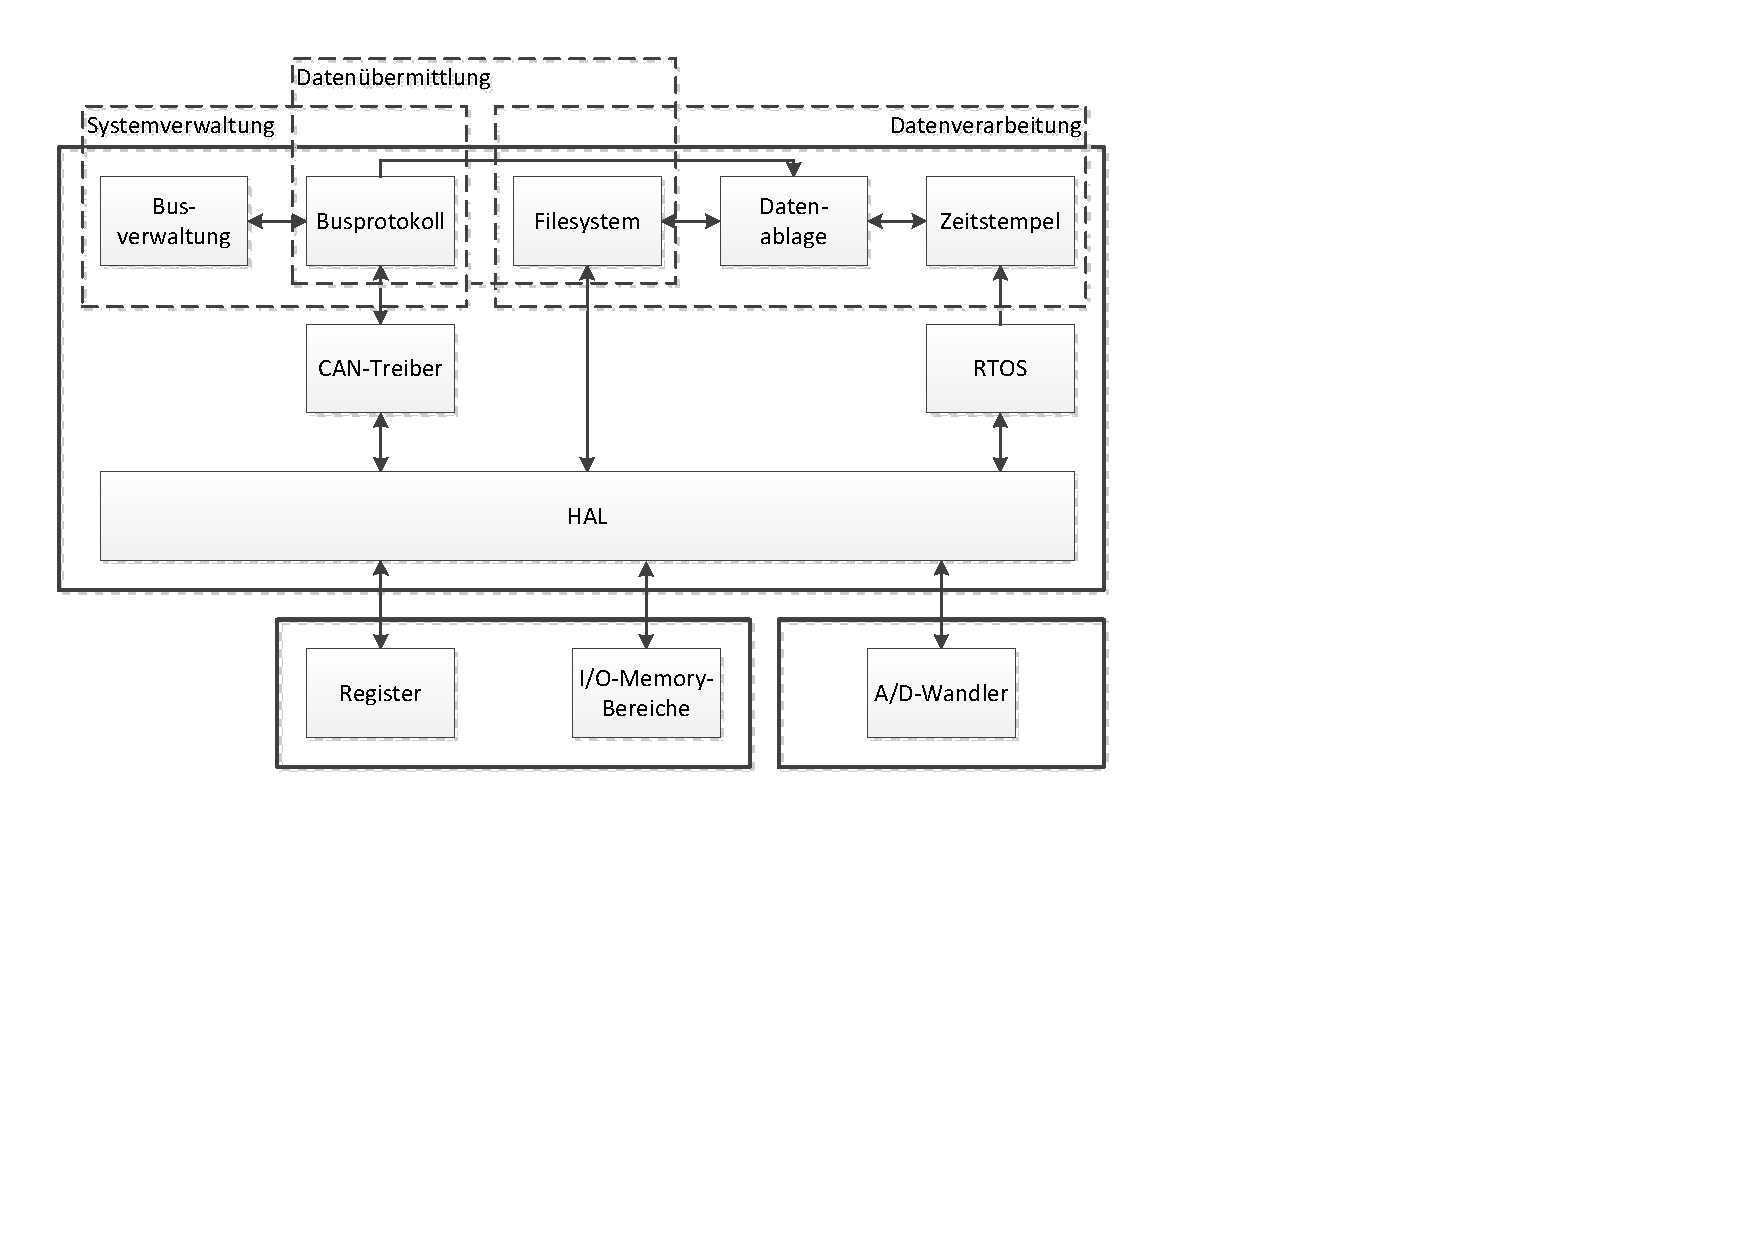
\includegraphics[width=0.8\textwidth]{images/visio/Softwarestack_Logger.pdf}
	\caption{Softwarestack des \gls{logger}s.}
	\label{fig.sw_logger}
\end{figure}

\begin{figure}
	\centering
		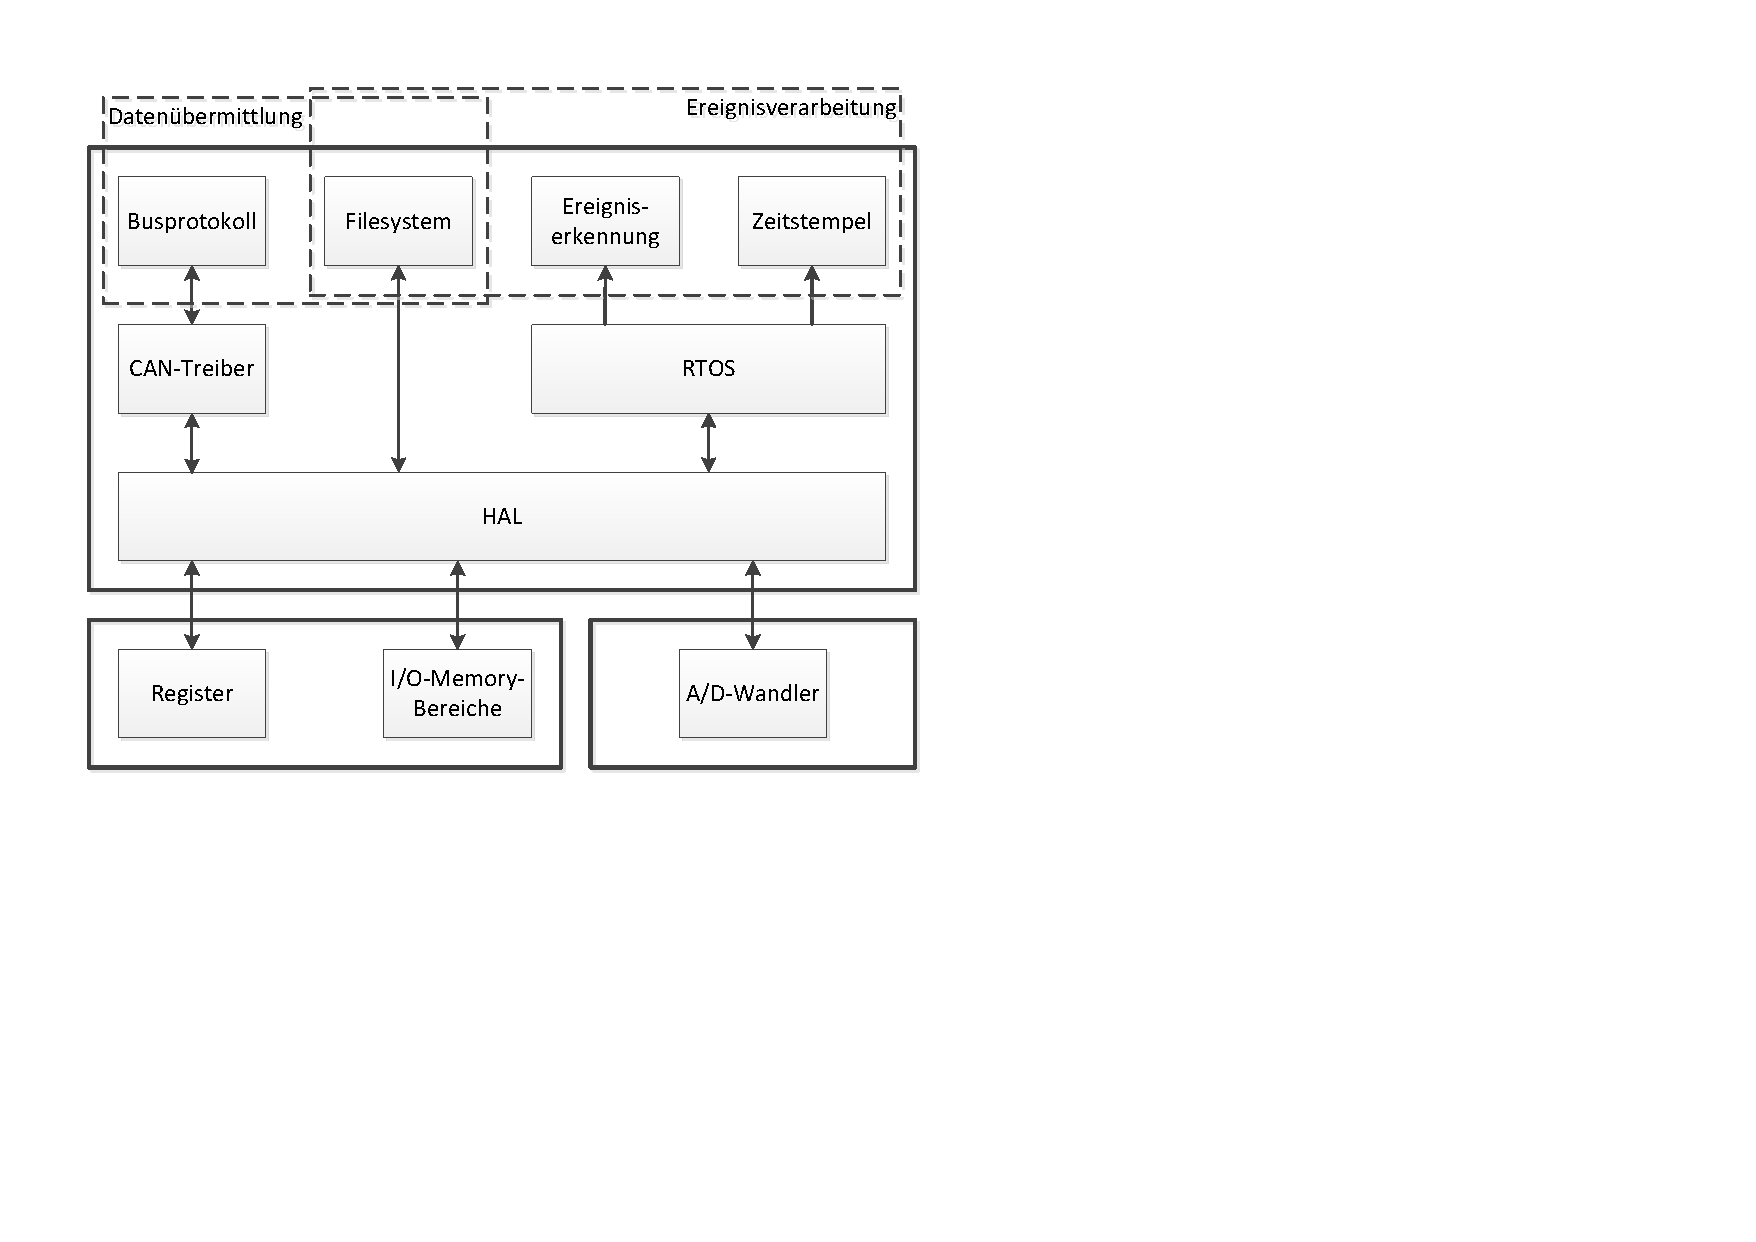
\includegraphics[width=0.8\textwidth]{images/visio/Softwarestack_Sensor.pdf}
	\caption{Softwarestack der \gls{sensoreinh}.}
	\label{fig.sw_sensor}
\end{figure}



\subsection{Messdatenerfassung}\label{subsec.sw_messen}
Der NXP LPC4088 Mikroprozessor verfügt über einen 12-bit A/D-Wandler, der über einen Multiplexer auf acht \glspl{pin} messen kann. Auf dem verwendeten Quickstart-Board stehen sechs \glspl{pin} für A/D-Wandlung zur Verfügung. Für die geplante Anwendung reicht ein A/D-Pin, da der Beschleunigungs-\gls{sensor} die Beschleunigung nur auf einer Achse misst. Der \gls{adwandler} des NXP LPC4088 wird mit einer \gls{fs} von 10~kHz betrieben. Falls höhere \glspl{fs} nötig sind, kann der \gls{adwandler} mit bis zu 400~kHz betrieben werden.

\todo{Prioritäten des Prozesse Messung, Erkennung, Übermittlung erklären, und wie wir das gelöst haben.}


\subsection{Ereigniserkennung}\label{subsec.sw_ereignis}
\subsubsection{Hilbert-Transformation}
Von der \gls{wsl} wurde die \gls{ereignisdet} bisher mittels \gls{hilbert} gelöst. Die \gls{hilbert} liefert die umhüllende Kurve des gemessenen \gls{signal}s. Überschreitet die Umhüllende den \gls{threshold}, markiert dies den Start eines neuen \gls{ereignis}ses. Fällt die Umhüllende unter den \gls{threshold}, ist das \gls{ereignis} beendet.

Die Berechnung der \gls{hilbert} erfordert einigen Aufwand. Mittels \gls{dft} wird das Spektrum des Signals berechnet. Negative Frequenzanteile werden auf null gesetzt und das resultierende Spektrum mittels \gls{idft} wieder in ein Signal umgerechnet \cite{wiki_hilbert}. Das resultierende Signal umhüllt das Eingangssignal. 
      \todo{figure: umhüllende (matlab: hilbert())} 
Für die \gls{dft} und die \gls{idft} ist der Rechenaufwand je \ensuremath{N \cdot log_2(N)}. Je mehr Datenpunkte in einem Schritt verrechnet werden (\gls{blockg}), desto höher ist der Aufwand, aber desto genauer ist das Resultat. Mit einer \gls{blockg} von 128 Messwerten benötigt die \gls{dft} und die \gls{idft} je 896 komplexe Multiplikationen und Additionen \cite[Kap. 3, S. 48]{dsv1_hilbert}. Pro Messwert sind das 7 komplexe Multiplikationen und Additionen. Dank der DSP-Fähigkeiten des gewählten Cortex\texttrademark -M4 Prozessors liegt die zu erwartende Prozessorauslastung für die \gls{hilbert} bei einer \gls{fs} von \ensuremath{10~kHz} bei wenigen Prozent.

\subsubsection{Hilbert-Transformation als FIR-Filter}
Die \gls{hilbert} kann mittels eines \gls{fir}s angenähert werden. Ein Allpass mit gerader Filter-Ordnung und geeignet gewählten Koeffizienten (Abbildung \ref{fig.hilbertFIR}) liefert eine gute Näherung. Je nach gewählter Ordnung des Filters ist der Rechenaufwand aber in ähnlicher Grössenordnung wie mit \gls{dft} und \gls{idft}.
\begin{figure}
	\centering
		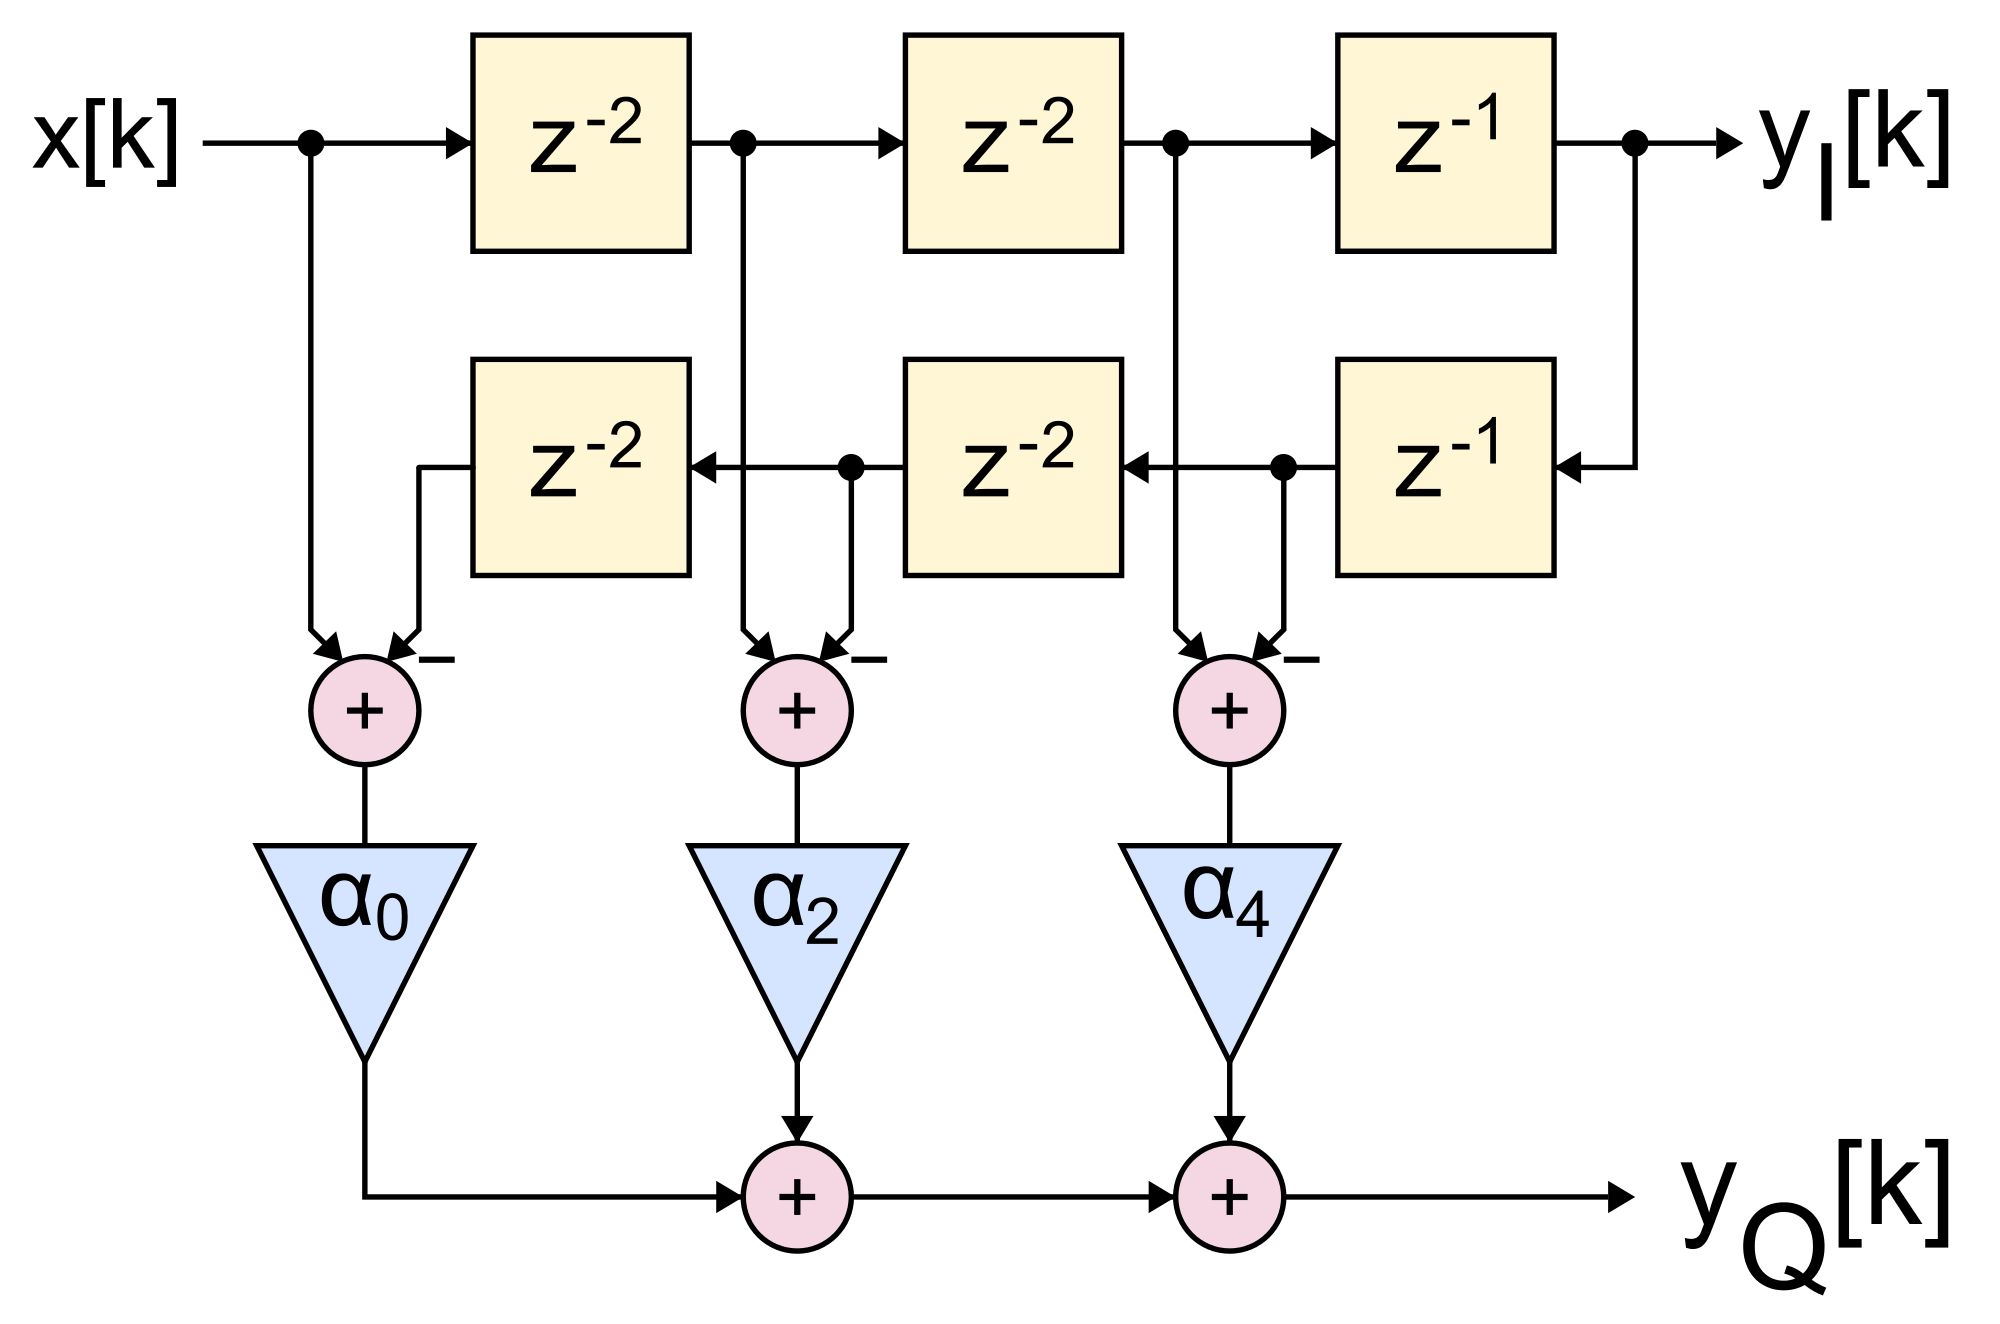
\includegraphics[width=0.8\textwidth]{images/FIR_Hilbert_Transform_Filter.png}
	\caption{\gls{hilbert} als \gls{fir} \cite{wiki_hilbertFIR}.}
	\label{fig.hilbertFIR}
\end{figure}

\subsubsection{Zustandsmaschine}
Um den Rechenaufwand der Hilbert-Transformation zu umgehen, lösen wir die \gls{ereignisdet} mittels einer \gls{fsm}. Das Zustandsdiagramm der \gls{fsmgloss} in Abbildung \ref{fig.fsm_impact_detection} zeigt alle möglichen Zustände der \gls{fsm} und welche Ereignisse einen Übergang in einen anderen Zustand auslösen.
\todo{Ereignis-FSM anpassen auf neue Stati}
\begin{figure}
	\centering
		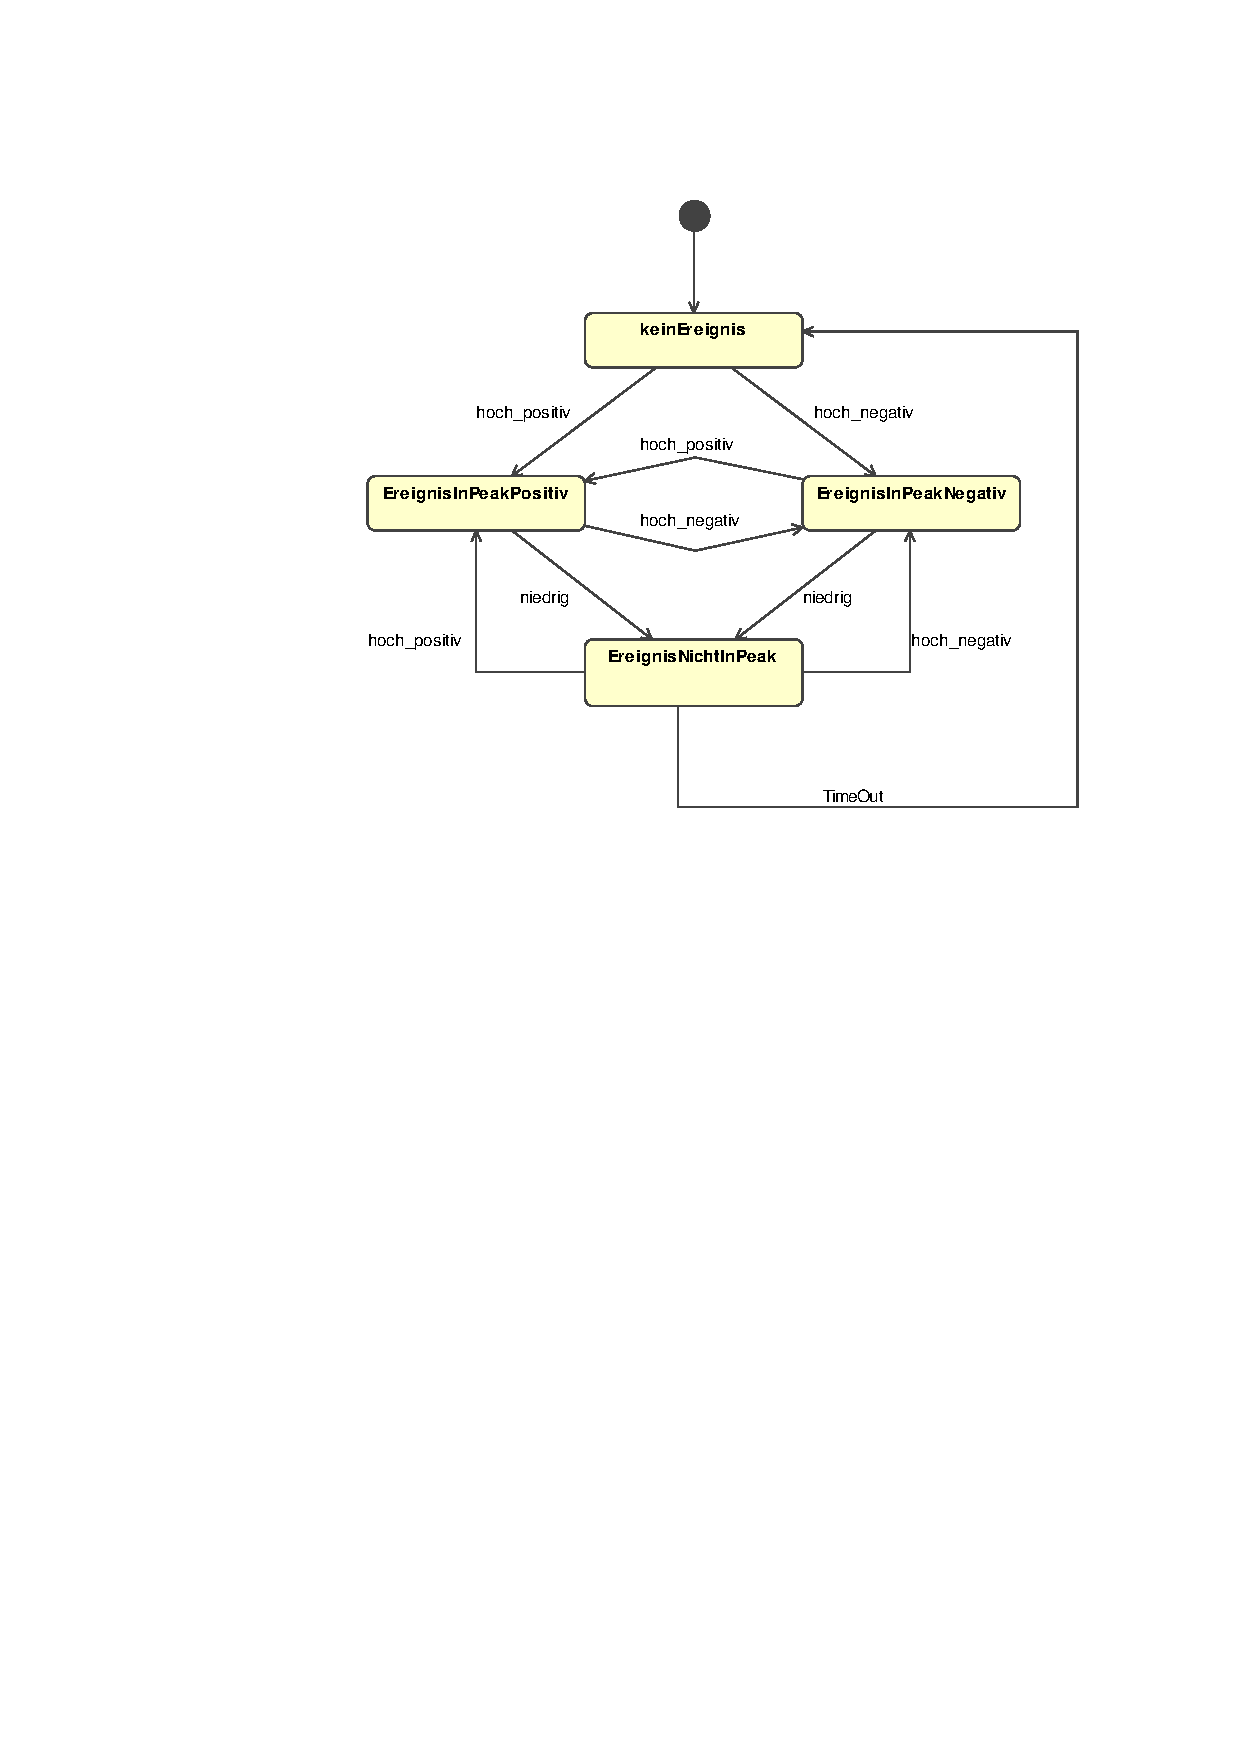
\includegraphics[width=0.8\textwidth]{images/magicdraw/Ereigniserkennung.pdf}
	\caption{Zustandsmaschine der Ereigniserkennung.}
	\label{fig.fsm_impact_detection}
\end{figure}

\paragraph{Konfiguration der Zustandsmaschine}
 Über Parameter wird definiert, welche Signalform als \gls{ereignis} erkannt werden soll. In Abbildung \ref{fig.impact_detection_params} sind die Parameter dargestellt. 
\begin{figure}
	\centering
	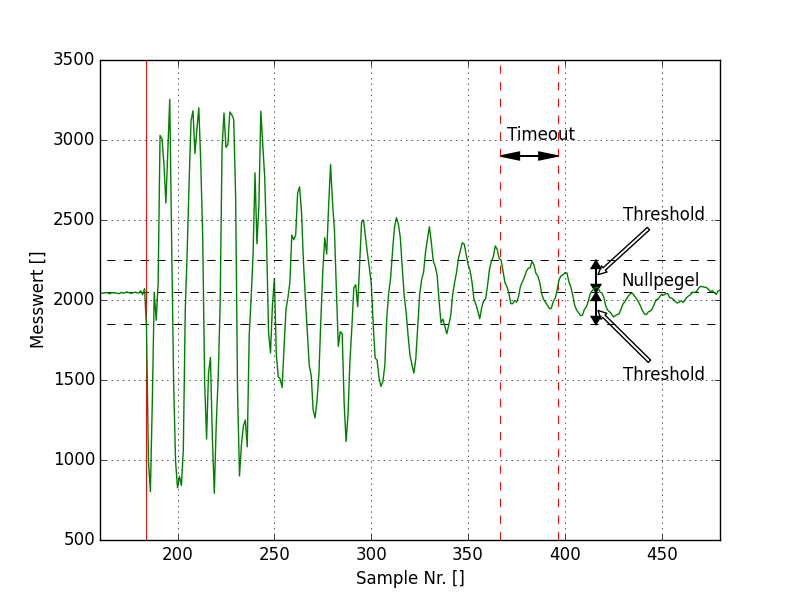
\includegraphics[width=0.8\textwidth]{images/impact_params.png}
	\caption{Parameter der Ereigniserkennung.}
	\label{fig.impact_detection_params}
\end{figure}
\paragraph{Nullpegel} Der \gls{nullpegel} kann angepasst werden, um die Erdanziehung, die als Beschleunigung auf den Sensor wirkt, zu kompensieren. Je nachdem wie der Sensor orientiert ist, ist die Erdanziehungskraft nicht parallel zur Mess-Achse des Sensors und damit nicht in jedem Fall gleich gross. Deshalb muss dieser Wert angepasst werden können.
\paragraph{threshold} Der \gls{threshold} definiert, ab welcher Abweichung des Signalpegels vom Nullpegel die \gls{fsm} einen Messwert als 'hoch' betrachten soll. Zu beachten ist, dass der \gls{threshold} auf beide Seiten des Nullpegels gilt. Da der Sensor sowohl Beschleunigungen nach oben wie auch nach unten erfährt, unterscheidet die \gls{fsm} dies mit den Ereignissen 'hoch\_positiv' resp. 'hoch\_negativ'. Signalpegel, die den Threshold nicht überschreiten, werden als 'niedrig' eingestuft.
\paragraph{Timeout} Da ein Ereignis nicht nur aus einem \gls{peak} besteht, muss eine Dauer (\gls{timeout}) definiert werden können, während der die \gls{fsm} auf den Beginn eines neuen \gls{peak}s wartet. Tritt während des \gls{timeout}s kein neuer Peak auf, gilt das Ereignis als beendet.

\subsubsection{Ablauf der Zustandsmaschine}
Im Folgenden wird der Ablauf in der Zustandsmaschine genauer erklärt. Im Zustandsdiagramm in Abbildung \ref{fig.fsm_impact_detection} sind die Namen der Zustände und Ereignisse ersichtlich. Der Übersichtlichkeit halber wurde auf die Auflistung der Aktionen im Diagramm verzichtet.

Die \gls{fsm} wird im Zustand 'keinEreignis' initialisiert. Tritt ein Messwert auf, der als 'hoch\_positiv' klassiert wird, wechselt die \gls{fsm} in den Zustand 'EreignisInPeak\_positiv'. In diesem Zustand verbleibt die \gls{fsm}, bis ein anders klassierter Messwert eintrifft. 

Ein Messwert 'niedrig', also unterhalb des \gls{threshold}s, führt zu einem Übergang in den Zustand 'EreignisNichtInPeak'. Dieser Übergang startet einen Timer, der während der im Parameter 'Timeout' definierten Anzahl Messwerte läuft. Falls die \gls{fsm} bis zum Ablauf des Timers keinen Messwert 'hoch\_positiv' oder 'hoch\_negativ' erhält, wechselt sie wieder in den Zustand 'keinEreignis' und übergibt die Ereignisdaten dem Prozess, der für die Übertragung zum \gls{logger} zuständig ist. 

Der Timer läuft nicht in Echtzeit, sondern zählt die Anzahl Messwerte seit seinem Start, da die Verarbeitung asynchron zur Erfassung der Messwerte läuft. Das bedeutet, dass die Verarbeitung problemlos während mehreren Messwerten stillstehen kann, ohne dass Messwerte verloren gehen. Dies ist möglich, da die Messwerte in eine Warteschlange (Queue) geschrieben werden, von wo sie von der \gls{fsm} abgeholt werden. So lange die Queue nicht überfüllt wird, gehen keine Messwerte verloren. Die Verarbeitung der Messwerte in der \gls{fsm} erfolgt im NXP LPC4088 Prozessor schnell genug, um theoretisch mit einer \gls{fs} bis \ensuremath{200~kHz} messen zu können.
\todo{Meldung ins Busprotokoll für den Verlust von Messwerten!}

\todo{Zusammenhänge A/D-Wandlung und Ereigniserkennung und Übertragung beschreiben, dazu ein Kommunikationsdiagramm, wo synchron, wo asynchron.}

\todo{Verschiedene Betriebsmodi mit Grafiken beschreiben}
\todo{Berechnungen, in welchem Modus wie lange gemessen werden kann, und wie lange ein \gls{sensor} mit dem vorhandenen Speicher die Resultate zwischenspeichern kann. Allenfalls ein System erwähnen, das automatisch zwischen verschiedenen Modi hin- und herschalten kann. (Ist allerdings heikel). Wie viele \glspl{sensor} können in welchem Modus gleichzeitig am System betrieben werden, bei welcher Ereignisrate ist Schluss mit Busbandbreite.}

\subsection{\gls{timestamp}}\label{subsec.sw_timestamp}
\todo{Timestamp beschreiben, Rechnung über die Dauer der eindeutigen Zuweisung.}

\subsection{Verwaltung der Messstation}\label{subsec.sw_busverwaltung}
\todo{Busverwaltung beschreiben}

\begin{figure}
	\centering
		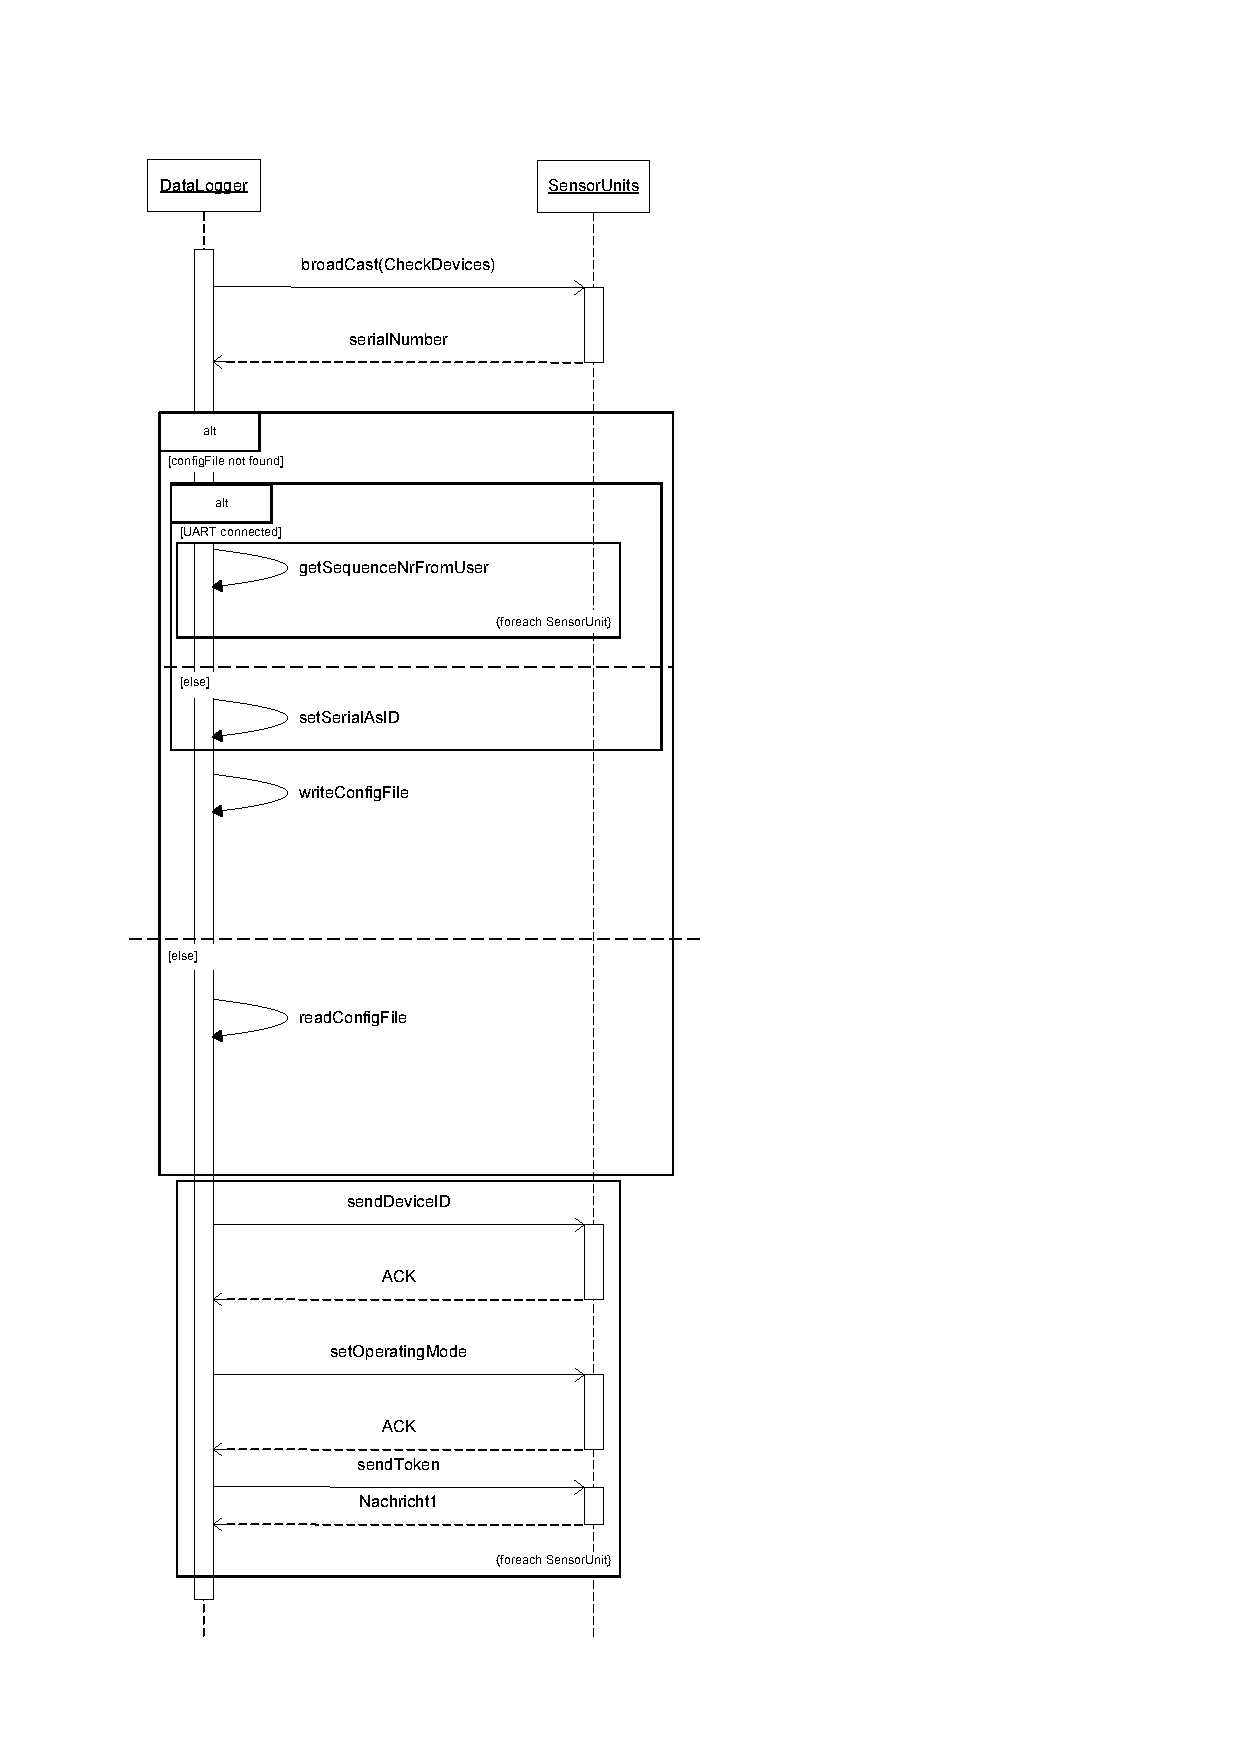
\includegraphics[height=0.9\textheight]{images/magicdraw/StartUpSequenz.pdf}
	\caption{Sequenzdiagramm des Startupvorgangs der Messstation.}
	\label{fig.seq_startup}
\end{figure}

\todo{Figur \ref{fig.seq_startup} aufteilen auf zwei Seiten. (PDF-crop)}

\subsection{Busprotokoll}\label{subsec.sw_busprotokoll}
\todo{Busprotokoll austüfteln. Darstellung siehe HW-Konzept Rioxo, genaue Beschreibung der Nachrichtentypen. Timestamp der einzelnen Peaks bezieht sich auf Offset vom Beginn des Impacts.}
\todo{Kommunikationsdiagramm Bushandler}
\todo{Interrupt-System des Bushandlers aufführen}

\subsection{Filesystem}\label{subsec.sw_filesystem}
\todo{Texten}
\todo{Frage: wird für jeden \gls{sensor} ein eigenes File geführt? Kann man alle Files offen lassen oder ist das keine gute Idee? Was ist besser, jedes mal das File-Ende zu suchen um neues anzuhängen?}

\subsection{UART-Kommandozeile}\label{subsec.sw_uart}
\todo{Dokumentation über die Kommandos, wird später für die Bedienungsanleitung gebraucht}

\section{Funktionalität}\label{sec.sw_funktionalitaet}
\todo{Texten}

\section{Konfiguration}\label{sec.sw_konfiguration}
\todo{Hier eine Art Bedienungsanleitung zur Konfiguration geben. Welches Kommando hat was 
zur Folge? (Wird Datenerfassung neu gestartet, werden allenfalls andere \glspl{sensor} deaktiviert 
etc.}

\section{Parallele Prozesse}\label{sec.parallel}